\documentclass[10pt,twocolumn,letterpaper]{article}
\usepackage{array}
\usepackage{statcourse}
\usepackage{times}
\usepackage{epsfig}
\usepackage{graphicx}
\usepackage{amsmath}
\usepackage{amssymb}
\usepackage{booktabs}
\usepackage{multirow}
\usepackage{hyperref}
% Include other packages here, before hyperref.

% If you comment hyperref and then uncomment it, you should delete
% egpaper.aux before re-running latex.  (Or just hit 'q' on the first latex
% run, let it finish, and you should be clear).

\statcoursefinalcopy%

\setcounter{page}{1}
\begin{document}


%%%%%%%%%%%%%%%%%%%%%%%%%%%%%%%%%%%%%%%%%%%%%%%%%%%%%%%%%%%%%%%
% DO NOT EDIT ANYTHING ABOVE THIS LINE
% EXCEPT IF YOU LIKE TO USE ADDITIONAL PACKAGES
%%%%%%%%%%%%%%%%%%%%%%%%%%%%%%%%%%%%%%%%%%%%%%%%%%%%%%%%%%%%%%%



%%%%%%%%% TITLE
\title{Comparative Analysis of Machine Learning Models: \\Alexnet, VGG, Resnet, YOLO}

\author{Pham Duc An\\
{\tt\small 10422002}
\and
Tran Hai Duong\\
{\tt\small 10422021}
\and
Vo Thi Hong Ha\\
{\tt\small 10421015}
\and
Nguyen Hoang Anh Khoa\\
{\tt\small 10422037}
\and
Truong Hao Nhien\\
{\tt\small 10422062}
\and
Nguyen Song Thien Phuc\\
{\tt\small 10422067}\\
\\
\{\tt @student.vgu.edu.vn\}
\and
Bui Duc Xuan\\
{\tt\small 10422085}
}

\maketitle
%\thispagestyle{empty}



% MAIN ARTICLE GOES BELOW
%%%%%%%%%%%%%%%%%%%%%%%%%%%%%%%%%%%%%%%%%%%%%%%%%%%%%%%%%%%%%%%


%%%%%%%%% ABSTRACT
\begin{abstract}
        In this project, we conducted a comprehensive comparative analysis of prominent machine learning models, namely Alexnet, VGG, Resnet, and YOLO, with a focus on their efficacy in image recognition. Leveraging a curated dataset representative of diverse real-world scenarios with CIFAR-10, our study delved into the nuances of each model's architecture, training process, and computational requirements. Through rigorous evaluation using metrics such as accuracy, precision, and recall, our results reveal nuanced performance distinctions. Notably, Resnet demonstrated superior accuracy, VGG excelled in feature extraction, YOLO showcased real-time efficiency, and Alexnet exhibited a stable performance. These findings provide valuable insights for practitioners and researchers seeking to optimize model selection for specific applications, shedding light on the trade-offs between accuracy, computational cost, and real-time processing capabilities. Project's detailed code are provided at {\url{https://github.com/nhientruong04/LIA-introCS-proj}}.
\end{abstract}

%%%%%%%%% BODY TEXT
\subsection{AlexNet}
In 2012, the ImageNet Large Scale Visual Recognition Challenge (ILSVRC) \footnote{\url{https://image-net.org/challengehttps://image-net.org/challenges/LSVRC/index.phps/LSVRC/index.php}} dataset was introduced, which required a model capable of processing a large dataset like ImageNet. The introduction of Alexnet by Alex Krizhevsky, Ilya Sutskever, and Geoffrey E. Hinton marked a significant milestone in the field of computer vision. Alexnet showed the feasibility of deep learning so well that it got a top-five error of fifteen point three percent on data that has a thousand categories in the ILSVRC 2012\cite{krizhevsky_2012_imagenet}. Its original paper is the theoretical basis for the report below.
\subsubsection{Overall architecture}

Human cognitive processes, mirroring the intricacies of an advanced supercomputer\cite{hassan2019computer}, rely on the nuanced interaction of neurons to perceive diverse stimuli such as digits, numbers, words, and images. This cognitive evolution spans from its early stages to the present era, with a notable milestone being the introduction of not only Generative AI but also other groundbreaking advancements in artificial intelligence.

In an era defined by the rapid advancement of artificial intelligence, the field of machine learning and deep learning stands as a beacon of innovation, transforming the way computers perceive and interact with their surroundings. This project delves into the intricate world of these cutting-edge technologies, specifically focusing on computer vision—a domain crucial for tasks ranging from image recognition to object detection. With the four chosen prominent models-Alexnet\cite{alex2012deep}, VGG\cite{simonyan2015deep}, Resnet\cite{he2015deep}, and YOLO\cite{yolov5}, we are seeking to unravel the complexities and reveal the engine behind these widely recognized models.

The comprehensive AI taxonomy proposed by IBM outlines seven distinct types, with Generative AI representing the initial stride in the AI continuum. Within this evolving landscape, Convolutional Neural Networks (CNNs)\footnote{\url{https://arxiv.org/pdf/1511.08458.pdf}} have garnered particular attention and proven to be a pivotal model. CNNs stand out for their remarkable application in various domains, excelling in tasks such as image classification, object detection, and pattern recognition.

\begin{flushleft}
    \begin{figure}[h!]
    \begin{center}
        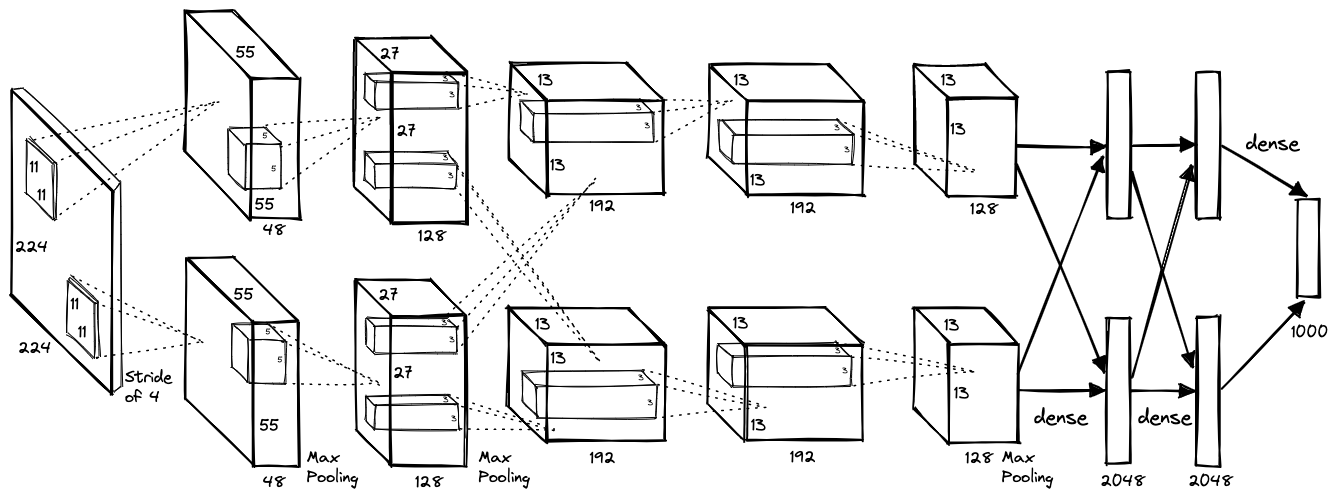
\includegraphics[scale=0.15]{imagenet-6}
        \caption{An illustration of the architecture of}{AlexNet\footnote{The input size is mentioned at most of the places as 224*224*3 but due to some special reason which happens it works out to be 227*227*3.}}{, clearly demonstrating the division of responsibility between the two GPUs.}
        \label{fig:imagenet-6}
    \end{center}
    \end{figure}
\end{flushleft}
Alexnet is a deep convolutional neural network that has 8 layers with learnable parameters. It consists of 5 convolutional layers and 3 fully connected layers. The first two Convolutional layers are followed by the pooling layers which are used to perform max pooling. The third, fourth, and fifth convolutional layers are connected directly. The Alexnet architecture takes images of size 227*227 as input and has three layers based on the RGB. After going through each layer, the number of filters becomes the kernels in the output feature map. The structure involves an increase in the number of filters as we go deeper into the architecture. The filter size is also reduced, which means the initial filter was larger. The first layers can recognize simple features, like edges, shapes, and textures. As the network gets deeper, it produces more abstract representations, eventually identifying concepts from mammals to dogs and even Siberian huskies \cite{shipra_2021_alexnet}. In the end, fully connected layers are used to produce the 1000-label classification needed for ImageNet. The output of the last fully-connected layer is fed to a 1000-way softmax which produces a distribution over the 1000 class labels\cite{krizhevsky_2012_imagenet}.



\subsubsection{ReLu activation function}

\begin{flushleft}
    
\begin{figure}[h!]
    \begin{center}
        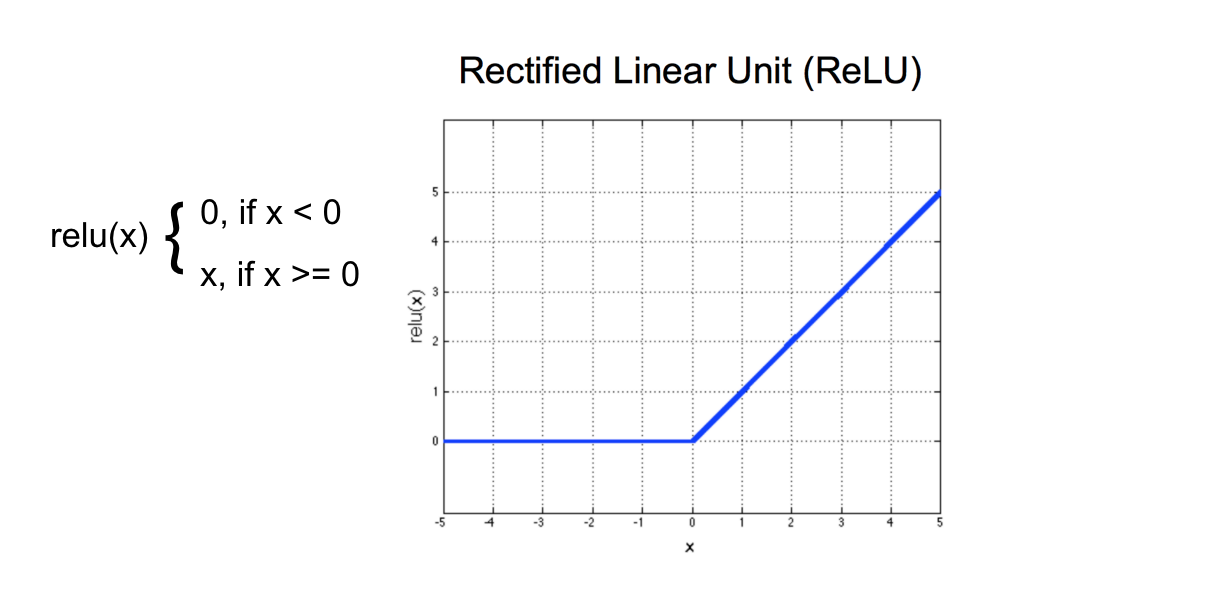
\includegraphics[scale=0.35]{relu_ex}
        \caption{ReLU activation function in the}{positive interval is always 1.}
        \label{fig:relu_ex}
    \end{center}
\end{figure}
\end{flushleft}
The AlexNet architecture introduced the use of ReLU (Rectified Linear Unit) Nonlinearity, which is a more efficient activation function than the previously used Tanh or sigmoid functions. It can be represented as: f(x) = max(0, x), where x is the input value. The paper shows that using ReLUs, AlexNet could achieve a 25\% training error rate six times faster than an equivalent network using tanh. This was tested on the CIFAR-10 dataset\cite{krizhevsky_2012_imagenet}. The function is applied after all the convolution and fully connected layers.

\subsubsection{ Multi(2)-GPU learning}
Multi-GPU learning is a method that allows for the parallelization of the training process across multiple GPUs. The authors utilized two GPUs to increase the network size, as the GPU at that time had a memory limit of 3GB. The network is split into two such as Figure \ref {fig:imagenet-6}, which communicated in specific layers to ensure they were not training two separate models. Therefore, the two-GPU net takes slightly less time to train than the one-GPU net.

\subsubsection{Dropout}
Dropout is a regularization technique that helps to prevent overfitting by randomly setting some neurons to zero during the training process. In AlexNet, dropout is applied to the first two fully-connected layers with a dropout rate of 0,5. This means that half of the neurons in these layers are ignored during each iteration of training. Dropout helps to improve the generalization performance of AlexNet on large-scale image recognition tasks.

\begin{flushleft}
    
\begin{figure}[h!]
    \begin{center}
        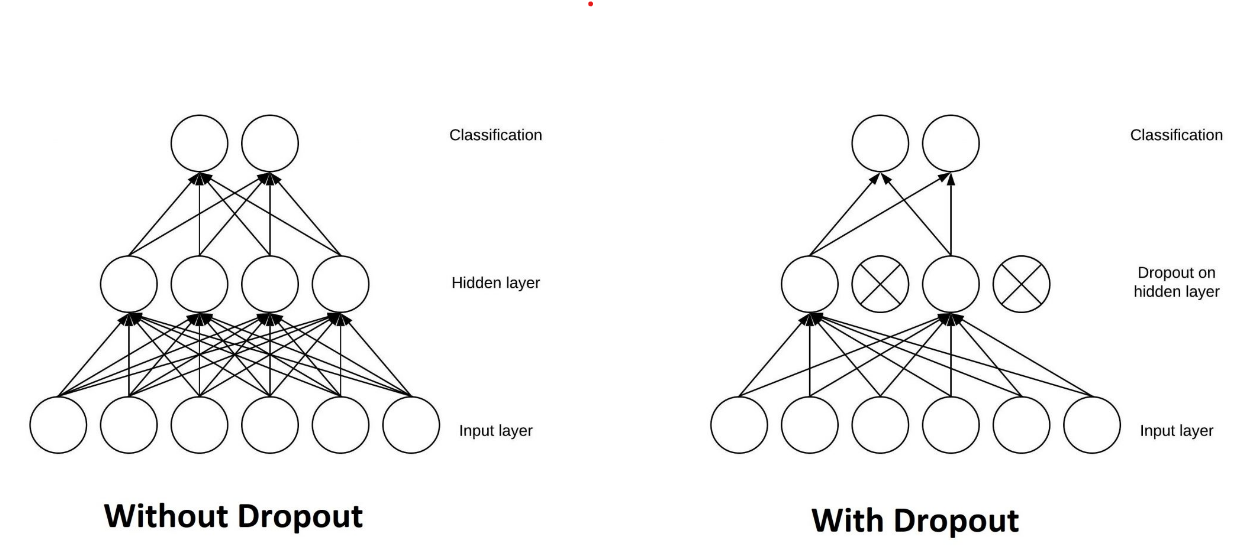
\includegraphics[scale=0.3]{dropout}
        \caption{Dropout Neural Net Model\cite{baeldung_2020_how}.}
        \label{fig:dropout}
    \end{center}
\end{figure}
\end{flushleft}



\paragraph{Literature review} Before delving into the specific machine learning models, it is crucial to contextualize this study within the existing body of knowledge. The literature review section provides a comprehensive overview of relevant research, identifying key advancements, methodologies, and challenges in the field of image recognition and machine learning. By synthesizing existing literature, we aim to establish a foundation for understanding the evolution of these models and highlight gaps that our study seeks to address.

\paragraph{Models} The following section explores four machine learning models-Alexnet, VGGNet, ResNet, and YOLO\@. We delve into their architectures, training nuances, and some key highlight that makes each of the models different.

\paragraph{Challenges} Despite the remarkable strides made in the development of machine learning models, challenges persist. In this section, we identify and discuss key challenges encountered in the deployment and optimization of these models, offering insights into areas that demand further attention.

\paragraph{Experiments} The experiment section outlines the experimental setup, including the dataset, evaluation metrics, and implementation details. We then present the results of our experiments, highlighting the nuances of each model's performance.

\paragraph{Conclusion} Summarizes findings, highlighting nuanced performance distinctions, and discusses implications for practitioners. Outlines potential avenues for future research.


\section{Literature review}

Deep learning methodologies have been widely applied in the detection and classification of images, with a multitude of research focusing on improving their precision and effectiveness. Each research study is unique, considering factors such as the specific type of tasks, the deep learning methods used, the performance metrics applied, and the datasets chosen. These factors could potentially affect the applicability of the models to different datasets. By categorizing these studies based on the specific type of tasks and the deep learning method used, we can identify similarities and differences, which could provide valuable insights for our current research. A significant number of studies have utilized convolutional neural networks (CNN) for object classification. For example, Krizhevsky et al.\cite{Alexnet} demonstrated the power of deep convolutional neural networks with AlexNet, a CNN with 8 convolutional layers and shows that it achieves a top-1 error rate of 15.3\% on the ImageNet classification task. This success paved the way for the development of deeper CNNs such as VGG and ResNet. Simonyan et al.\cite{VGG}  present a novel architecture for convolutional neural networks (CNNs) that enables the training of extremely deep networks (VGGNets)  and achieved state-of-the-art results,with a top-1 error rate of 5.1\% on the ImageNet classification task. Similarly, Zhang et al.\cite{ResNet} introduced the Deep Residual Learning (DRL) framework, which achieves record-breaking results  attaining a 3.57\% top-1 error rate for 152 layers on the ImageNet classification task. DRL introduces residual connections, which allow for the construction of much deeper networks without vanishing gradients. Despite these promising results, these CNNs models are limited in training and data related. Some studies employ other pipelines which include advanced techniques to get a better result in classification. Redmon et al.\cite{Yolo} used an unified framework algorithm, YOLO\@. With the assistance of the framework, it performs both object detection and classification in a single pass of the input image. YOLO is able to execute within a short period of time, while achieving comparable accuracy. These four models have been extensively studied and evaluated in the literature. For example, a comprehensive review of deep learning models for object detection by Vaswani et al. (2020)\cite{Review} compared the performance of AlexNet, VGG, ResNet, and YOLO on a variety of object detection datasets. The review found that ResNet and YOLO generally outperformed AlexNet and VGG on all datasets. These models have been shown to achieve state-of-the-art results on a variety of image recognition and object detection tasks. However, AlexNet, VGG, ResNet, and YOLO are still widely used in practice due to their simplicity, robustness, and accuracy.


\section{Insightful summarization}


\begin{table}[h]
        \centering
        \label{tab:small_table}
        \scalebox{0.7}{\begin{tabular}{|c|c|c|c|c|}
                        \hline

                        Models      & Release Date & Number of layers & Params (M) & Flops(G)\footnote{} \\
                        \hline
                        AlexNet     & 2012         & 8                & 61         & 0.715               \\
                        VGGNet      & 2014         & 16 or 19         & 138-144    & 15.5-20             \\
                        ResNet-50   & 2015         & 50               & 25.56      & 4.12                \\
                        ResNet101   & 2015         & 101              & 44.55      & 7.85                \\
                        Yolov5x-cis & 2020         & 19               & 48.1       & 15.9                \\
                        Yolov8x-cls & 2023         & 53               & 57.4       & 154.8               \\
                        \hline
                \end{tabular}}
        \caption{Data Comparision}
\end{table}
\footnotetext{GigaFlop (or Gflop) is a billion FLOPS. Here we take the data of the models that train with ImageNet dataset}

In addition to the aspects mentioned above, models that were created afterwards fixed the weaknesses of their predecessors. For instance,  AlexNet lacks explicit regularization techniques, making it prone to overfitting. VGGNet incorporates dropout, a regularization technique that randomly drops out a certain percentage of neurons during training. This forces the model to learn more robust and generalizable features, reducing overfitting and improving generalization performance. Although AlexNet implies dropout as well but only in the first two fully connected layers, VGGNet has it in both convolutional and connected layers. However, these two plain networks still confront the degradation problem when it comes to extending their architectures. Hence, Resnet was made to solve the vanishing gradients problem as the layers went deeper and deeper. Yolo is more like a pipeline that includes CNN models as backbone and others applies advanced techniques into training. Leading to a significant increase in FLOPs in terms of the numbers of params.

\section{Models}

\subsection{ResNet}
ResNet is an innovative result realized by a team of Microsoft researchers during participating the ILSVRC 2015, with the ultimate grand achievement is the first place of the competition by using multiple ensembles rooted from ResNet. Its original paper \cite{ResNet}, has gained substantial citations and is considered one of the most important contributions in the field of Computer Vision.

\subsubsection{Addressed problems}

\paragraph{Main problems} With the rapid development of convolutional neural networks after the success of VGGNet \cite{VGG}, various networks have been created based on the idea of VGG, “the deeper, the better”. Despite multiple slight differences in terms of layers or activation functions in those models, the same technique aiming at creating a model that was “deep enough” was utilized popularly at that time. However, a new problem was raised questioning the “deepness” of any CNN models: “How deep can a model be extended?”. The problem is called the degradation phenomenon, when a deeper version of a CNN model performs worse than its shallower counterparts. This experiment was shown in the paper of Resnet, when the authors trained 2 plain models and compared their performance, as shown in \ref{fig:Resnet_intro}. It is clear that the 20-layer model performed better than its deeper counterpart in both training and testing set. This graph also showed that the degradation phenomenon was not correlated with the overfitting problem \cite{overfitting_overview}, as the training error of the 56-layer model was higher than the 20-layer one and no divergence between the training error and the testing error was found. The authors argued that this phenomenon is caused when an already sufficiently deep model gets deeper, then its accuracy and training error would saturate earlier instead of achieving its efficient local extremum.

\begin{figure}
        \begin{center}
                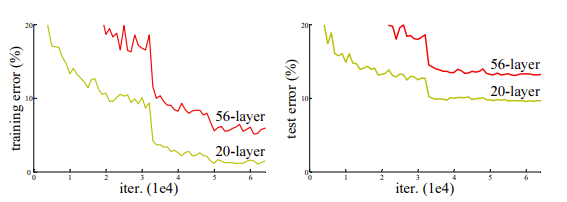
\includegraphics[width=0.45\textwidth]{figures/resnet_intro_compare.png}
                \caption{Training error (left) and test error (right) on CIFAR-10
                        with 20-layer and 56-layer “plain” networks. The image was taken from the ResNet paper \cite{ResNet}.}
                \label{fig:Resnet_intro}
        \end{center}
\end{figure}

\paragraph{The pitfall of vanishing gradients} The degradation phenomenon mentioned above is currently still a controversial topic, when many sources \cite{visoai, Datagen_2023,GeeksforGeeks_2023} agree that this phenomenon is rooted from the vanishing gradients problem \cite{exp_vanishing_grad_1,exp_vanishing_grad_2}. This is indeed a valid reason since the gradients would gradually decay through each individual layer in the backpropagation phase. However, the authors of ResNet argued that the vanishing gradients problem has little effect on the model causing the degradation phenomenon. “We argue that this optimization difficulty is unlikely to be caused by vanishing gradients. These plain networks are trained with BN, which ensures forward propagated signals to have non-zero variances. We also verify that the backward propagated gradients exhibit healthy norms with BN. So neither forward nor backward signals vanish.”, stated by Kaiming He et al. in their paper \cite{ResNet}. Based on this argument, they argued that the degradation phenomenon was indeed a natural dilemma arising from the action of deepening any CNN models. This argument directly opposes the effect of the vanishing gradients problem on deep models, which would require that more proof and experiments must be conducted to approve any sides. However, despite the different reasoning of the degradation phenomenon, one of the same goals of any models created till now is avoiding this problem.

\subsubsection{Architecture}

\paragraph{Skip connections} Mathematically, defining a residual block with a skip connection as:
\[y=\uppercase{\gamma}(x) + x\]
With \(\uppercase{\gamma}(x)\) represents a generalized convolutional mapping with an activation function. The equation strictly illustrates combining input \(x\) with \(\uppercase{\gamma}(x)\) through addition expression. A skip connection is a pathway for any input feature map to flow to the output of the next layer. The intuition behind this technique resembles the process of a person reviewing a picture one more time that has not seen for a long time. Adding the input to the output feature map is believed to make the model “remember” its input, since any processing or calculation that input went through may make the output completely unrelated. Moreover, many sources of information about ResNet besides the authors agree that these skip connections will alleviate the vanishing gradients problem, hence could help the model to have a greater amount of layers.

\begin{figure}
        \begin{center}
                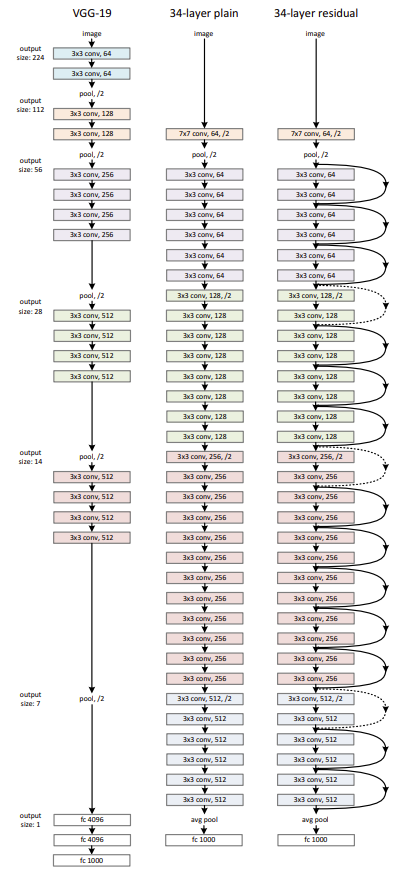
\includegraphics[width=0.4\textwidth]{figures/resnet_architecture.png}
                \caption{Architecture of ResNet compared to plain models. The image was taken from the ResNet paper \cite{ResNet}.}
                \label{fig:Resnet_architecture}
        \end{center}
\end{figure}


\paragraph{The general architecture} Since skip connections can be used as an identity mapping in any CNN models, the proposed ResNet would have many layers, from 34 to 151 layers preferably. The skip connections are utilized in each layer, as shown in \ref{fig:Resnet_architecture}. The proposed ResNet model resembles the VGGNet in terms of using small kernel size for convolutional layers and stacking a sufficient amount of these layers. The skip connections can be directly used when the input and output are of the same dimensions (solid line shortcuts in \ref{fig:Resnet_architecture}). When the dimensions increase (dotted line shortcuts in \ref{fig:Resnet_architecture}), there are 2 options: (A) The shortcut still performs identity mapping, with extra zero entries padded for increasing dimensions. This option introduces no extra parameter; (B) The projection shortcut is used to match dimensions (done by 1×1 convolutions). For both options, when the shortcuts go across feature maps of two sizes, they are performed with a stride of 2.

\subsubsection{Applications}

The invention of ResNet sparks the utilization of that same structure, especially the skip connections or residual blocks, in many CNN models not only in the Computer Vision field but also a greater, older field which is Natural Language Processing. Some impactful architectures developed based on ResNet are ResNeXt \cite{ResNeXt} and DenseNet \cite{DenseNet}, where residual blocks and skip connections are implemented differently to tackle the weaknesses of ResNet. In addition, those skip connections (or preferably called identity mapping), are utilized in Transformer \cite{Transformer}, which is an evolutionary architecture that outperformed any forms of CNN in NLP. The same architecture was also widely used to create different types of Transformer models in the Computer Vision field, such as ViT \cite{ViT} or Swin \cite{Swin}. The skip connections used in Transformer sequentially made the Attention blocks in this model a new type of residual blocks.


\section{Agile Scrum in Brief}
Agile Scrum is a dynamic project management framework designed for teams developing complex products. Rooted in Agile principles, Scrum emphasizes iterative progress, collaboration, and adaptability. With roles like Product Owner, Scrum Master, and Development Team, Scrum fosters clear communication and shared ownership. Key ceremonies, such as Sprint Planning and Daily Scrum, keep the team focused, and artifacts like the Product Backlog ensure transparent progress. Agile Scrum is widely used for its ability to deliver incremental value, respond to change, and enhance overall project efficiency.

\section{Development Cycle}

In the dynamic landscape of project management, the Agile framework, particularly Scrum, has emerged as a beacon for teams seeking efficient, collaborative, and adaptable work methodologies. Our 5-week Scrum journey began with an ambitious goal: exploring the convergence of CNNs and AI models for performance comparison. Over the course of five weeks, we carefully followed the Scrum workflow to discover three different AI models—Yolo, AlexNet, VGG, and ResNet. This method guided us through the exploration, smoothly transitioning from research and scoping to the implementation phase.

\subsection{Week 1: Research and Project Scope Definition (22/10 - 28/10)}
This week was pivotal as we delved into extensive research, culminating in the definition of our project scope and the formation of three specialized teams, each dedicated to a distinct AI model: YOLO, AlexNet, VGG, and ResNet. Here are ours activities:

\paragraph{Research Exploration} The week started with a thorough exploration of the details of CNNs and how they are used in AI. Team members conducted extensive research, examining the strengths, weaknesses, and specific applications of well-known models like YOLO, AlexNet, VGG, and ResNet. This phase was essential for gaining a detailed understanding of the varied capabilities these models bring to the table.

\paragraph{Project Scope Definition}
Building on the insights gained from the research phase, the team collaborated to define the project scope. Clear and concise objectives were outlined, emphasizing the unique contributions that each AI model could make to the overarching project. This step ensured that the team had a unified vision, setting the direction for the subsequent sprints.

\paragraph{Team Formation}
With the project scope defined, the next step was to form specialized teams, each assigned to one of the chosen AI models. This approach allowed for a focused and in-depth exploration of each model's capabilities. The YOLO team, the AlexNet team, the VGG team, and the ResNet team were formed, with members possessing complementary skills and expertise.

\paragraph{Initial Sprint Planning}
To kick off the Scrum framework, the teams engaged in initial sprint planning sessions. Tasks were allocated based on individual strengths, ensuring a balanced distribution of responsibilities. The teams set the groundwork for the upcoming sprints, aligning their efforts with the overarching project goals.

\subsection{Week 2: First Implementation and Model Training (29/10 - 4/11)}
With our project scope defined and teams divided, the second week of our 5-week Scrum journey marked the initiation of the implementation phase. This stage focused on the practical application of our research findings as we began the process of training each AI model—Yolo, AlexNet, VGG, and ResNet.

\paragraph{Model Training Sessions}
A significant portion of the week was dedicated to hands-on model training sessions. Each specialized team delved into the specifics of training their assigned model, exploring parameters, and optimizing configurations. This phase was crucial for refining our understanding of the practical nuances associated with YOLO, AlexNet, VGG, and ResNet.

\paragraph{Continuous Learning and Adaptation}
As the model training progressed, our teams embraced a culture of continuous learning and adaptation. Daily stand-ups became forums for sharing insights, addressing challenges, and refining strategies. This iterative approach allowed us to adjust our methods in real-time, ensuring optimal outcomes during the implementation phase.

\paragraph{Documentation and Progress Tracking}
At the same time, keeping detailed records and tracking our progress were crucial during this implementation phase. Every team documented their training steps, noted any changes, and recorded significant results. This not only gave us a reference for future use but also added transparency and accountability to the entire project.

\subsection{Week 3: Parameter Adjustment and Model Comparison (5/11 - 11/11)}
In the third week of our 5-week Scrum expedition, our focus shifted to fine-tuning the parameters of each AI model and conducting a comprehensive comparison. This crucial phase aimed to optimize the performance of YOLO, AlexNet, VGG, and ResNet while facilitating an insightful evaluation of their individual strengths and weaknesses.

\paragraph{Parameter Fine-Tuning}
The week kicked off with teams delving into the meticulous process of adjusting parameters for each AI model. This fine-tuning aimed to enhance the models' efficiency, accuracy, and overall performance. Iterative adjustments were made based on the feedback loop established in the preceding weeks.

\paragraph{Comparative Analysis}
With the models optimized, the teams engaged in a rigorous comparative analysis. This involved evaluating the performance metrics, such as precision, recall, and processing speed, to discern the distinctive features and trade-offs of YOLO, AlexNet, VGG, and ResNet. Comparative analysis sessions provided valuable insights into the practical implications of each model.

\paragraph{Team Collaboration on Findings}
Recognizing the significance of collaboration, teams convened to share their findings and insights. Cross-team discussions facilitated a broader understanding of the nuanced aspects of each model's performance. This collaborative approach encouraged the pooling of knowledge and contributed to a holistic view of the comparative results.

\paragraph{Adaptation to Insights}
As comparative analysis unfolded, teams embraced an adaptive mindset, ready to make further adjustments based on the comparative insights gained. The iterative nature of the Scrum framework allowed for dynamic responses to emerging observations, ensuring continuous improvement in the performance of YOLO, AlexNet, VGG, and ResNet.

\paragraph{Documentation of Comparative Results}
Similar to the preceding weeks, a focus on clear documentation persisted. Teams meticulously recorded the outcomes of the comparative analysis, noting significant findings, notable patterns, and any areas for potential refinement. This documentation not only served as a repository of knowledge but also facilitated informed decision-making as we progressed.

\subsection{Week 4: Presentation (12/11 - 18/11)}
Entering the fourth week of our 5-week Scrum expedition, our focus shifted to getting ready for the project presentation scheduled on 14/11/2023. This crucial week was all about putting together our findings, polishing our insights, and making sure our presentation on the convergence of CNNs and AI models was engaging and impactful.

\paragraph{Data Synthesis and Findings Clarification}
The week began with teams bringing together the information collected during the implementation, parameter adjustment, and model comparison phases. Findings were simplified into clear and straightforward points, showcasing the main insights from our exploration of YOLO, AlexNet, VGG, and ResNet.

\paragraph{Presentation Structure Planning}
Teams collaboratively planned the structure of the upcoming presentation. This involved outlining key sections, deciding on the sequence of model presentations, and allocating time for an effective delivery. The Scrum framework's emphasis on iterative planning facilitated a dynamic approach to refining the presentation structure.

\paragraph{Dry Runs and Feedback Sessions}
To ensure a successful presentation, teams rehearsed their parts, getting feedback and making adjustments internally. These practice sessions played a crucial role in refining the story, ensuring everything made sense, and handling any questions that might come up during the real presentation.

\paragraph{Reflection and Continuous Improvement}
At the same time, the week gave us a chance to have thoughtful discussions. Teams looked back on the entire journey, thinking about the challenges we dealt with, what we learned, and where we can get better. The Scrum framework's meetings to review and learn from our experiences were crucial in building a culture of always learning and getting better.

\paragraph{Finalizing the Report}
The week's activities ended with teams completing the presentation report. They combined their polished insights, brought together their findings, and added reflective observations to create a detailed document. This report not only acted as a guide for the presentation but also served as a tangible record of our 5-week Scrum journey.

\subsection{Week 5: Reflection and Report (19/11 - 25/11)}
In the last week of our 5-week Scrum journey, we turned our attention to creating the final report that captured everything we discovered about the convergence of CNNs and AI models. This week was crucial for summarizing our overall insights, lessons learned, and highlighting how our understanding evolved over the course of the journey.

\paragraph{Conclusion and Recommendations}
The final report had a strong conclusion summarizing the main findings and insights from our 5-week exploration. In addition, teams offered practical recommendations for future projects and improvements, showcasing the flexible and forward-thinking approach of the Scrum framework.

\paragraph{Peer Review and Feedback}
To ensure the report's quality, teams engaged in peer reviews and sought feedback from fellow team members. This collaborative process allowed for additional refinement, ensuring that the final report was comprehensive, accurate, and effectively communicated the essence of our journey.

\paragraph{Document Finalization}
The week concluded with the teams finalizing the report, incorporating feedback, and making any last-minute adjustments. This step marked the culmination of our 5-week Scrum journey, with the final report serving as a testament to our collaborative efforts and the outcomes of our exploration.

\section{Conclusion}

Considering Real-World Applications and Scenarios:
When assessing the performance of YOLO, ResNet, VGGNet, and AlexNet in image classification, it's essential to examine their suitability for real-world scenarios. Each model comes with distinct strengths and weaknesses, shaping their applicability across different use cases. Understanding these attributes is crucial for deploying these models effectively in practical applications.

\subsection{YOLO (You Only Look Once)}
Demonstrates notable efficiency and accuracy, particularly excelling in real-time object detection scenarios, prioritizing speed. It's important to note that YOLO operates as a pipeline, facilitating seamless and rapid processing in object detection tasks.

\subsection{ResNet}
Effectively addresses the vanishing gradient problem through deep residual learning, making it proficient in capturing intricate features, albeit demanding substantial computational resources.

\subsection{VGGNet}
Performs well in image classification tasks due to its straightforward design and consistent architecture, but may face challenges related to overfitting on large-scale datasets.

\subsection{AlexNet}
While an early deep learning architecture, AlexNet exhibits solid performance in image classification, though its design may be considered somewhat outdated compared to more recent models.

\subsection{Conclusive Remarks on the Most Effective Model for the Given Task}
In the context of image classification, considering the evaluated architectures, YOLO emerges as a strong performer. Its real-time object detection capabilities and high accuracy, coupled with its pipeline structure, position it as a favorable choice for scenarios where rapid and precise object identification is crucial.

\subsection{Future Directions for Research}
While YOLO stands out in image classification, there's room for ongoing research and improvement. Future endeavors could focus on optimizing the pipeline architecture for specific applications, enhancing adaptability to handle diverse object classes, and addressing identified limitations. Additionally, exploring ways to make YOLO more resource-efficient without compromising performance could broaden its deployment possibilities in resource-constrained environments.

In conclusion, this study offers insights into the comparative performance of YOLO, ResNet, VGGNet, and AlexNet in image classification tasks. The findings contribute to understanding these models and inform decision-making when selecting a suitable model for practical applications. YOLO's success, particularly as a pipeline, positions it as a promising option for image classification in real-world scenarios, with potential for further refinement and optimization in future research endeavors.

\section{Acknowledgement}

We would like to express our deepest appreciation to all those who provided us the possibility to complete this report. A special gratitude we give to Dr. Le Trong Nhan, whose contribution in stimulating suggestions and encouragement, helped us to coordinate our project especially in writing this report.

        {\small
                \bibliographystyle{ieee}
                \bibliography{bibliography.bib}
        }


\end{document}